    \documentclass{standalone}
\usepackage{tikz}
\usepackage{amsmath}         
\begin{document}
    \centering
    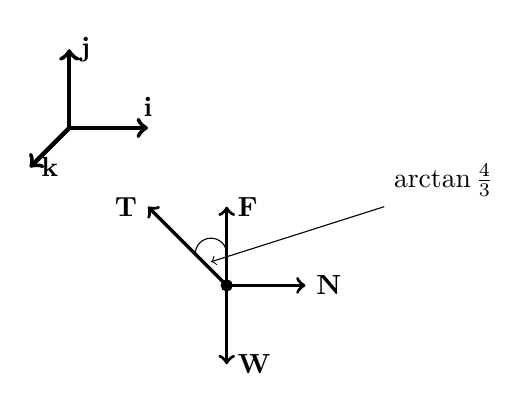
\begin{tikzpicture}
    [UnitVector/.style={ultra thick,->},
    force line/.style={very thick,->},
    dashed line/.style={dashed, thin},
    ]

    %vector
    \coordinate (VectorBase) at (-2,2);
    \draw[UnitVector] (VectorBase) -- +(1,0) node[above] {$\mathbf{i}$};
    \draw[UnitVector] (VectorBase) -- +(0,1) node[right] {$\mathbf{j}$};
    \draw[UnitVector] (VectorBase) -- +(-0.5,-0.5) node[right] {$\mathbf{k}$};

    %Particle
    \filldraw (0,0) circle (2pt);
    \draw[force line] (0,0) -- (0,-1) node[right]{$\mathbf{W}$};
    \draw[force line] (0,0) -- (-1,1) node[left]{$\mathbf{T}$};
    \draw[force line] (0,0) -- (0,1) node[right]{$\mathbf{F}$};
    \draw[force line] (0,0) -- (1,0) node[right]{$\mathbf{N}$};
    \draw (0,0.4) arc (0:180:0.2);
    \draw (2,1)[->]node[anchor=south west]{$\arctan\tfrac{4}{3}$}--(-0.2,0.3);

    \end{tikzpicture}
    \end{document}
